\section{Algorithme classique}

\begin{figure}[H]
    \centering
    \begin{minipage}{0.48\textwidth}
        \centering
        
\includegraphics[width=\textwidth]{11-Résultats/pic/classic/trajectoires.pdf}
        \caption{Trajectoire du barycentre de l'essaim}
        \label{fig:essaim_trajectory}
    \end{minipage}\hfill
    \begin{minipage}{0.48\textwidth}
        \centering
        
\includegraphics[width=\textwidth]{11-Résultats/pic/classic/trajectoires_marquage.pdf}
        \caption{Trajectoire de chaque robot de l'essaim}
        \label{fig:essaim_trajectory2}
    \end{minipage}
\end{figure}
\underline{Note :} Dans l’algorithme, l’essaim est considéré comme ayant atteint sa destination dès qu’il se trouve à moins de 5 cm du point-cible, ce qui explique les légères différences avec la trajectoire réelle tracée en bleu sur la Figure \ref{fig:essaim_trajectory}. Cette tolérance est conservée pour l’ensemble des méthodes évaluées. Exiger un arrêt exactement au point-cible conduirait souvent à des commandes trop faibles, absorbées par la zone morte des moteurs, immobilisant le robot et l’empêchant d’atteindre le point et bloquant l'essaim au complet. De plus, plus la précision exigée est grande, plus la vitesse de convergence est faible, ce qui allonge le temps nécessaire pour atteindre le point-cible.

Sur la Figure \ref{fig:inter_distances_classic}, les lignes en pointillés verticales représentent les moments où de nouveaux points-cible sont envoyés, et donc au moment où un point est atteint par l'essaim.

\begin{figure}[H]
    \vspace{-1cm}
    \centering
    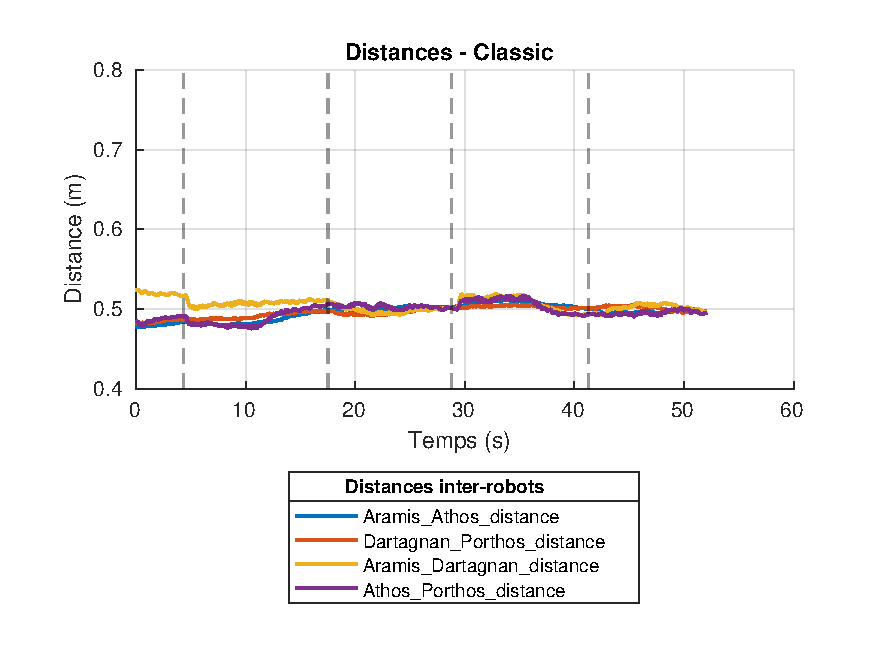
\includegraphics[width=0.8\textwidth]{11-Résultats/pic/classic/distance.pdf}
    \vspace{-0.5cm}
    \caption{Evolution des inter-distances entre les robots}
    \vspace{-0.3cm}

    \label{fig:inter_distances_classic}
    
\end{figure}
\noindent La formation et les interdistances sont maintenus tout au long du parcours.

Il est possible de tester la robustesse de l'algorithme en créant manuellement une perturbation. Pour cela, un robot (ici Athos) est déplacé à la main durant l'expérience de sorte à créer une erreur dans les inter-distances à maintenir.

\begin{figure}[H]
    \centering
    \begin{minipage}{0.48\textwidth}
        \centering
        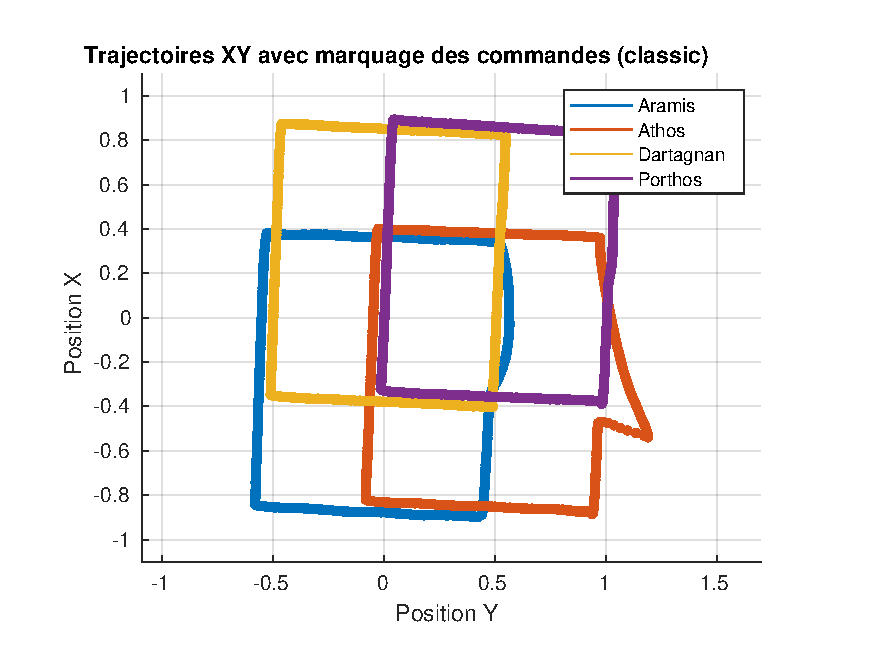
\includegraphics[width=\textwidth]{11-Résultats/pic/classic/perturbation/trajectoires_marquage.pdf}
        \caption{Trajectoire des robots avec une perturbation}
        \label{fig:essaim_trajectory2_perturbation}
    \end{minipage}\hfill
    \begin{minipage}{0.48\textwidth}
        \centering
        
\includegraphics[width=\textwidth]{11-Résultats/pic/classic/perturbation/distance.pdf}
        \caption{Evolution des inter-distances entre les robots avec perturbation}
        \label{fig:inter_distances_classic_perturbation}
    \end{minipage}
\end{figure}
\vspace{-0.2cm}

Il est possible d'observer sur la Figure \ref{fig:essaim_trajectory2_perturbation} que la perturbation sur le robot Athos provoque également une perturbation sur la trajectoire  d'Aramis (et aussi sur Porthos, mais moins visible, car pour corriger l'erreur, il doit se diriger selon $-x$, alors que sa trajectoire initiale est selon $+x$). Cela est logique, car ces robots sont voisins, et leurs trajectoires sont liées par les inter-distances à maintenir.
L'algorithme met environ 15 secondes pour corriger la perturbation (Figure \ref{fig:inter_distances_classic_perturbation}). Malgré la perturbation, l'essaim parvient à atteindre sa destination, et les inter-distances sont rétablies puis maintenues.
